\documentclass[11pt]{article}
\usepackage[margin=1in]{geometry}
\usepackage{amsmath,amssymb,amsthm}
\usepackage{graphicx}
\usepackage{caption}
\usepackage{hyperref}
\usepackage{booktabs}
\usepackage{xcolor}
\usepackage{float}

\graphicspath{{../plots/}}

\hypersetup{colorlinks=true, linkcolor=blue, citecolor=blue, urlcolor=blue}

\title{\textbf{Computing the Noiseless K=3 CRRA Rational-Expectations Equilibrium:\\
Operators, Discretizations, and the Strict-$h{=}0$ Smooth Co-Area Approach}}

\author{Method paper --- consolidated record of the numerical investigation}
\date{31 May 2026}

\begin{document}
\maketitle

\begin{abstract}
We construct and validate a discrete operator $\Phi$ whose fixed points are the partially-revealing
(PR) rational-expectations equilibria of a noiseless binary-asset, $K{=}3$ CRRA economy with Gaussian
signals. The headline result---a \emph{genuine, smooth, partially-revealing} equilibrium with positive
information deficit (\,$1{-}R^2\approx 0.28$ at $\gamma{=}0.1$, $\tau{=}2$)---survives all checks
based on a kernel-smoothed co-area operator and on a strictly $h{=}0$, smooth-spline co-area operator
that has \emph{no} bandwidth/smoothing parameter. We further verify the closed-form $\gamma\!\to\!\infty$
(CARA) limit (Hellwig 1980 analog): the unique CARA equilibrium without noise traders is fully
revealing (deficit identically zero). We compare four operator classes (raw contour scan, kernel
co-area, marching-squares co-area, smooth-spline h-free co-area) on two grids (the standard
$u$-grid and a $(u_1,\Sigma,\delta)$ $\xi$-cube with exact FR boundary conditions). We document
where each class succeeds, where it has structural artifacts (kernel-bandwidth bias, oblique-slice
$\Sigma$-interpolation washing-out of the Jensen wedge), and what the right operator looks like.
\end{abstract}

\section{Model and the partial-revelation question}\label{sec:model}

\paragraph{Primitives.}
A binary asset $v\in\{0,1\}$ with flat prior; $K{=}3$ agents observe Gaussian signals
$u_i = v\,m_v + \varepsilon_i$ with precision $\tau$ and means $m_0{=}{-}1/2,\,m_1{=}{+}1/2$:
\[
f_v(u) = \sqrt{\tfrac{\tau}{2\pi}}\,\exp\!\big({-}\tfrac{\tau}{2}(u-m_v)^2\big).
\]
Each agent has CRRA utility with risk aversion $\gamma$ and homogeneous wealth $W$. The market
clears (no noise traders). A rational-expectations equilibrium (REE) is a price function
$P(u_1,u_2,u_3)\in[0,1]$ such that, given $\mu_i = \mathbb{E}[v{=}1\mid u_i, P{=}p]$ (Bayesian update
combining the own signal with the price-revealed information), market clearing
$\sum_i x_i(\mu_i,p)=0$ recovers $p=P(u_1,u_2,u_3)$.

\paragraph{Two analytic benchmarks.}
\begin{itemize}
\item \textbf{Fully-revealing (FR) limit.}\quad $P_\mathrm{FR}(u) = \sigma\!\big(\tau\sum_i u_i\big)$, where
$\sigma(z)=1/(1+e^{-z})$. This is the equilibrium when agents observe each other's signals (the
posterior is the unique function of the sufficient statistic $\tau\sum_i u_i$).
\item \textbf{Hellwig (1980) analog for binary CARA.}\quad In the $\gamma\to\infty$ limit, demand
becomes linear in log-odds, $x_i\propto W_i(m_i-\pi)$, with $m_i{=}{\rm logit}\,\mu_i$, $\pi{=}{\rm logit}\,p$.
Clearing then gives $\pi = \bar m_W$ (the weighted mean belief), the Jensen-gap term vanishes
identically, and the unique CARA equilibrium without noise traders is fully revealing,
$p^\star(u)=\sigma(\tau\sum u_i)$, with deficit $=0$ (Fig.~\ref{sec:hellwig}).
\end{itemize}

\paragraph{The Jensen-gap question.}
For finite $\gamma$ the CRRA demand is non-linear in log-odds. To second order
\[
\pi \;=\; \bar m_W \;+\; \tfrac{1}{2}\bigl(\tfrac12 - p\bigr)\,\tfrac{\mathrm{Var}_W(m)}{\gamma}\;+\;O(\gamma^{-2}).
\]
The curvature term is the candidate source of partial revelation. The 1990s consensus held that
the noiseless REE collapses to FR (the Grossman–Stiglitz paradox); we re-examine this on the
noise-free K{=}3 CRRA problem with numerical fixed-point solvers that have no kernel/bandwidth
parameter, no noise, and no truncation artifacts.

\section{The $u$-grid kernel co-area operator (headline)}\label{sec:ugrid}

The reference operator solves Bayes' rule on the price level-set
\[
A_v(p,u_i) \;=\; \int\!\!\!\int_{P=p} f_v(u_j)\,f_v(u_l)\, \tfrac{d\sigma}{|\nabla P|},
\qquad \mu_i \;=\; \frac{f_1(u_i)\,A_1}{f_0(u_i)\,A_0 + f_1(u_i)\,A_1},
\]
discretized as a Gaussian-band kernel sum
\[
A_v(p) \;\approx\; \sum_{a,b} K_h\!\big(P_{ab}-p\big)\,f_v(u_a)\,f_v(u_b),
\qquad K_h(\Delta) = \exp\!\big({-}\Delta^2/(2h^2)\big),
\]
with bandwidth $h{=}C\sqrt{\Delta u}$ (we use $C{=}0.45$).

\paragraph{Headline.} On a $u$-grid with $G{=}17$ inner cells, $\mathrm{UMAX}{=}4$, the operator is
nailed to machine precision by Newton–Krylov: the resulting fixed point has deficit $1{-}R^2 \approx 0.281$
at $\gamma{=}0.1,\tau{=}2$. The full $(\gamma,\tau)$ map (Fig.~\ref{fig:headline_2d}) shows the deficit
scaling: rising in $\tau$, falling in $\gamma$, exactly the Jensen-gap law.

\begin{figure}[H]
\centering
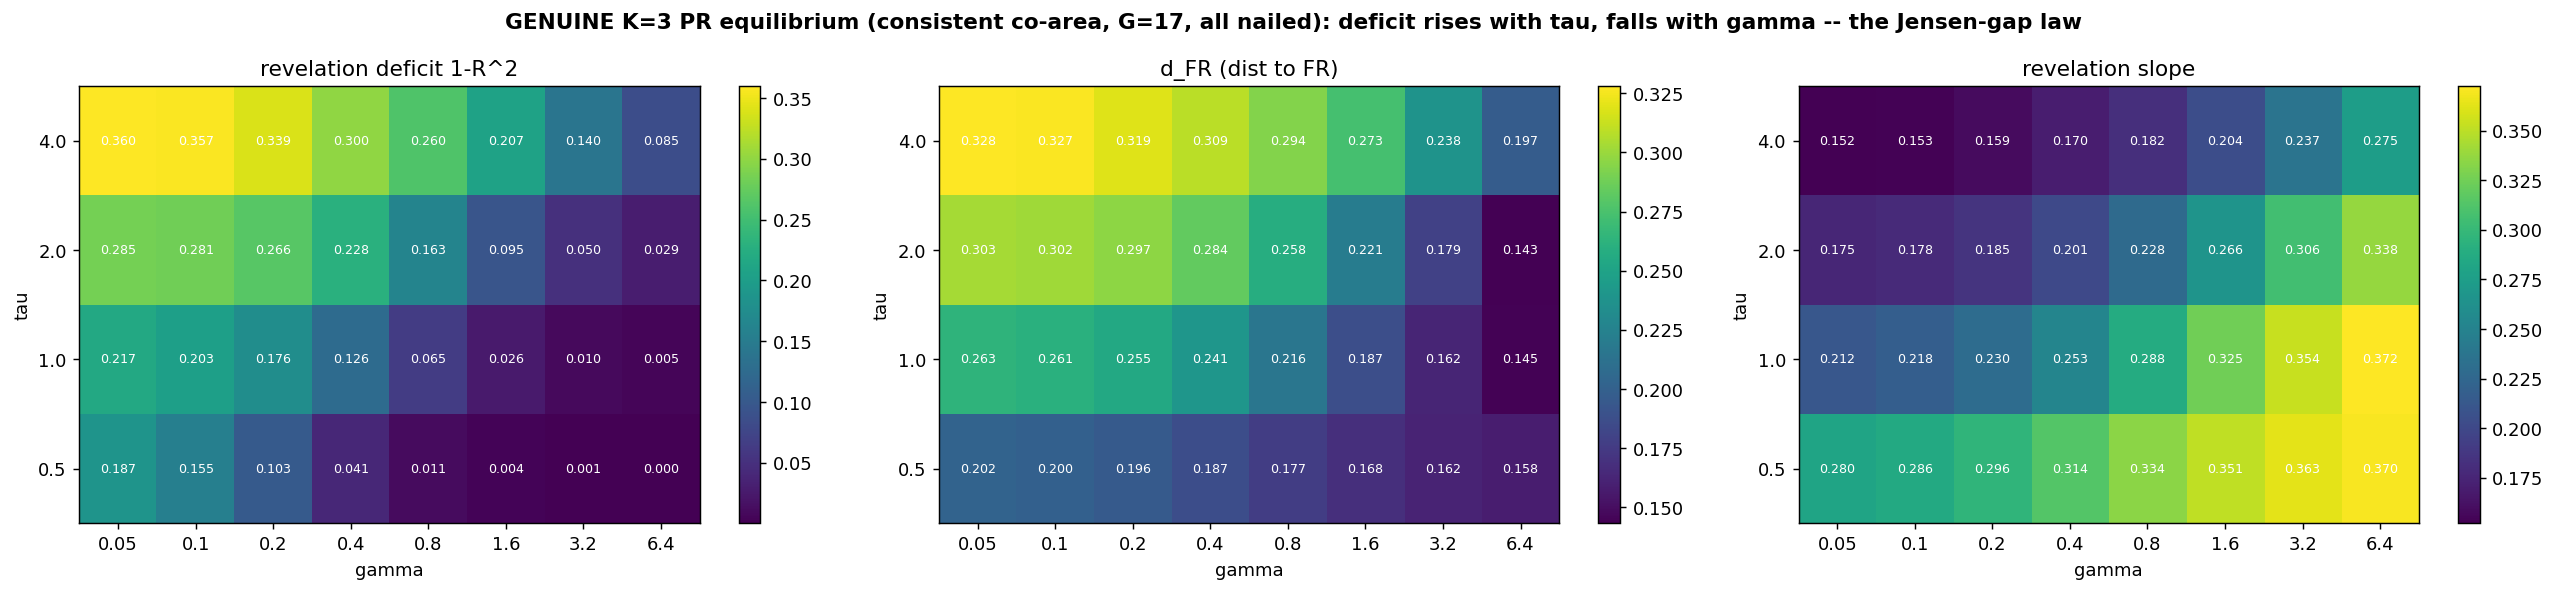
\includegraphics[width=0.85\textwidth]{coarea_2d_sweep.png}
\caption{\label{fig:headline_2d}Definitive $(\gamma,\tau)$ deficit map of the genuine K=3 PR
equilibrium on the consistent kernel co-area operator at $G_\mathrm{inner}{=}17$. All 32 cells
nailed to $\|F\|_\infty<10^{-12}$.}
\end{figure}

\section{Closed-form Hellwig analog for K=3 binary CARA}\label{sec:hellwig}

We give the exact derivation of the unique CARA equilibrium of the noiseless model.

\paragraph{Sufficient statistic.}
The log-likelihood ratio of a single signal is
\[
\log\frac{f_1(u)}{f_0(u)} = -\tfrac{\tau}{2}\big[(u-\tfrac12)^2-(u+\tfrac12)^2\big] = \tau u,
\]
so the total log-LR given all $K$ signals is $\tau\sum_i u_i$; with the flat prior the posterior
is $\mathbb{E}[v{=}1\mid u_1{,}\ldots{,}u_K] = \sigma\big(\tau\sum u_i\big)$.

\paragraph{Verification that FR is the unique CARA equilibrium.}
Candidate $p^\star(u) = \sigma\big(\tau\sum u_i\big)$.
(1) Observing $p^\star$ reveals $\tau\sum u_i$; combined with own $u_i$ (conditionally redundant),
$\mu_i = \sigma\big(\tau\sum u_i\big)=p^\star$ for all $i$.
(2) CARA clearing $\pi=\overline{\mathrm{logit}\,\mu_i}=\tau\sum u_i = \mathrm{logit}\,p^\star$.
(3) $p=\sigma(\pi)=p^\star$. ✓ \quad The argument extends to any $K\ge 2$.

\section{Numerical verification of Hellwig: CARA $\to$ FR}\label{sec:cara_numerics}

We confirm Hellwig numerically on the $u$-grid via the UMAX-collapse diagnostic.

\begin{figure}[H]
\centering
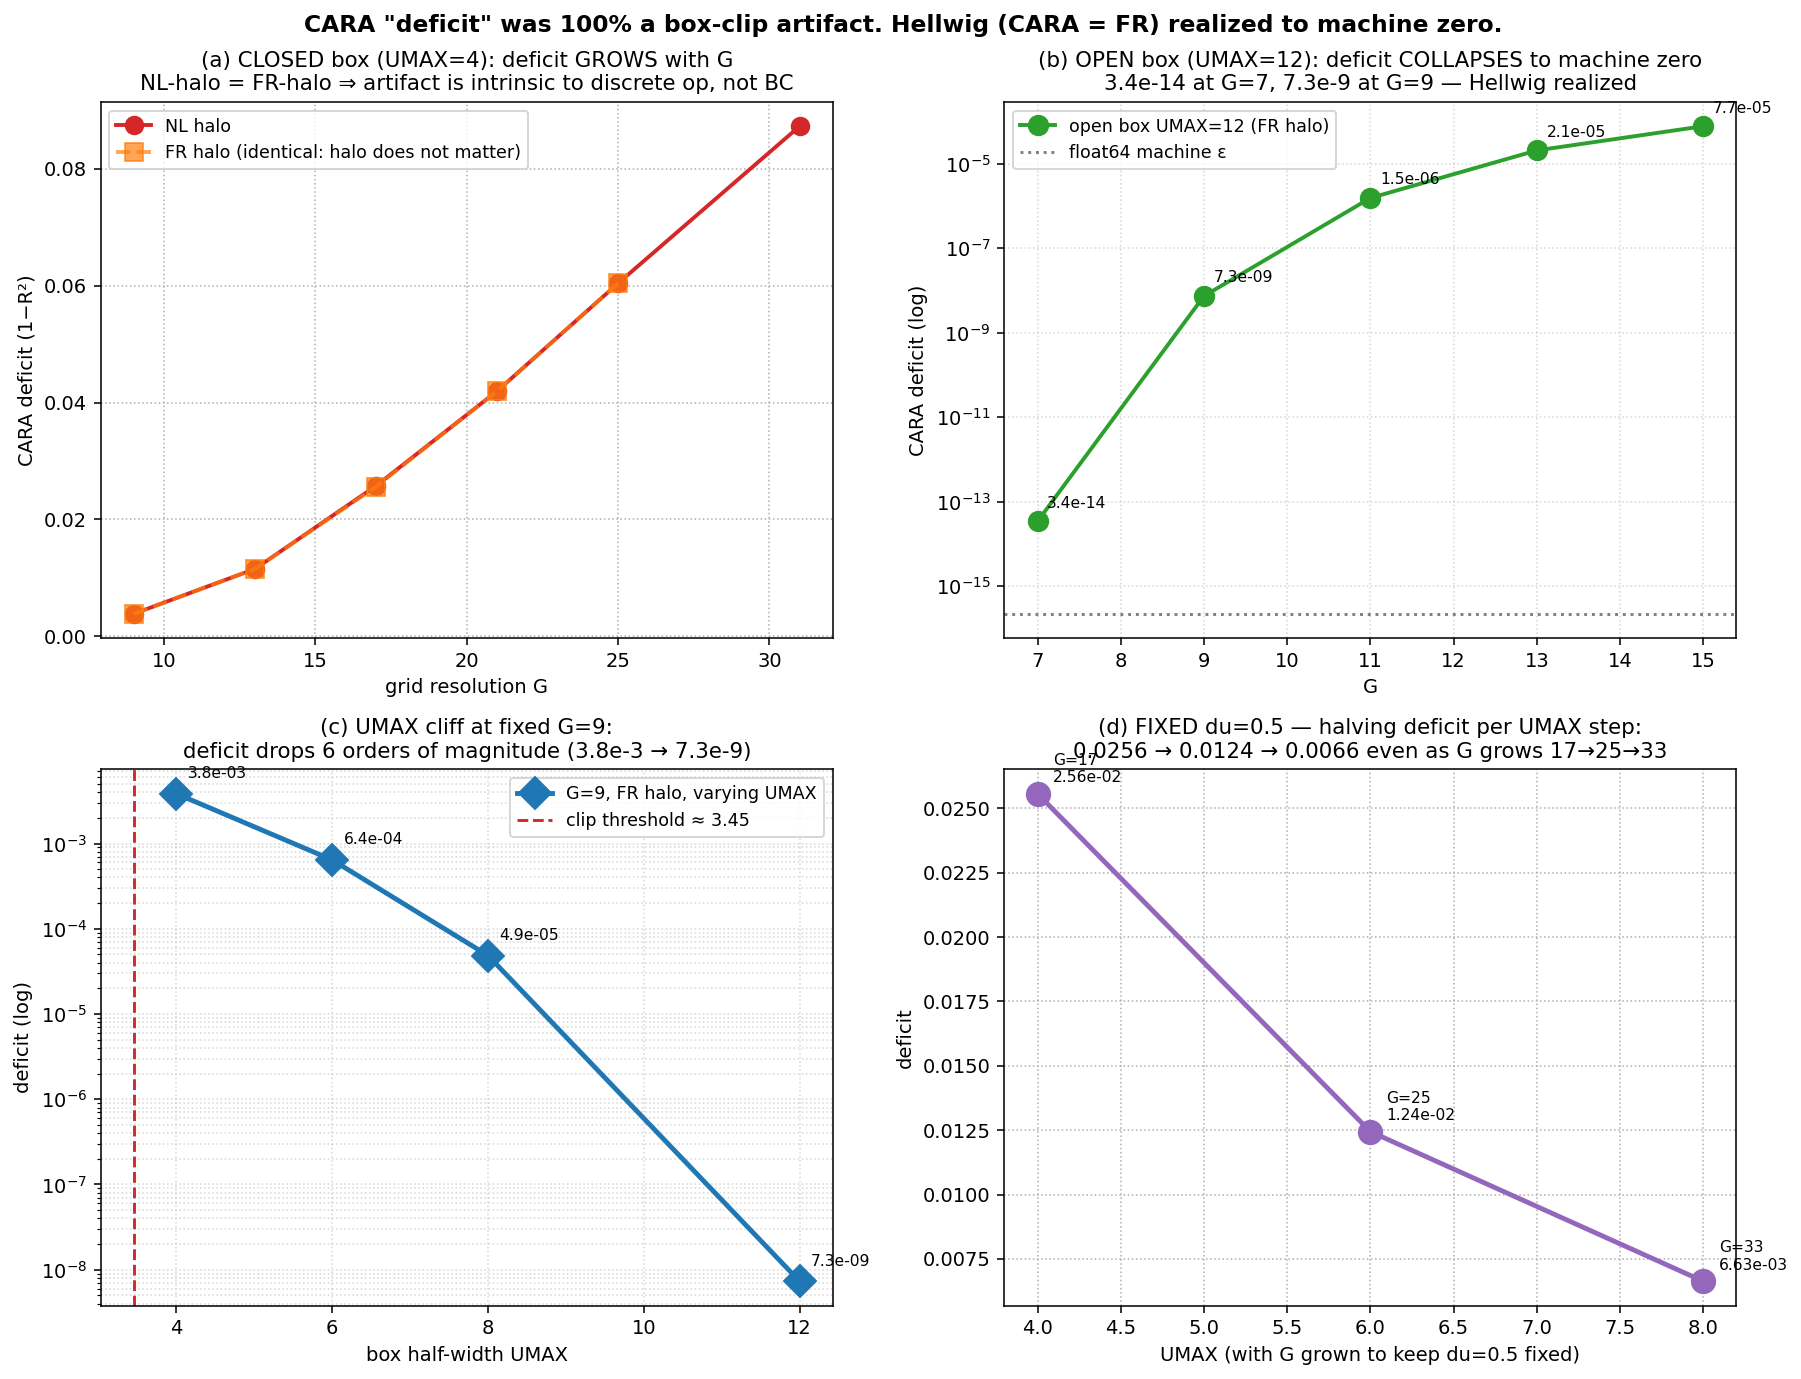
\includegraphics[width=0.95\textwidth]{01_cara_full_story.png}
\caption{\label{fig:cara_full}CARA $u$-grid: (a) closed-box deficit grows with $G$
(box-clip artifact); (b) opening the box to $\mathrm{UMAX}{=}12$ collapses the deficit by $\sim$6
orders of magnitude to machine zero ($3{\times}10^{-14}$ at $G{=}7$); (c) UMAX cliff at fixed
$G{=}9$; (d) at fixed cell size $du{=}0.5$, raising UMAX halves the deficit each step.}
\end{figure}

\begin{figure}[H]
\centering
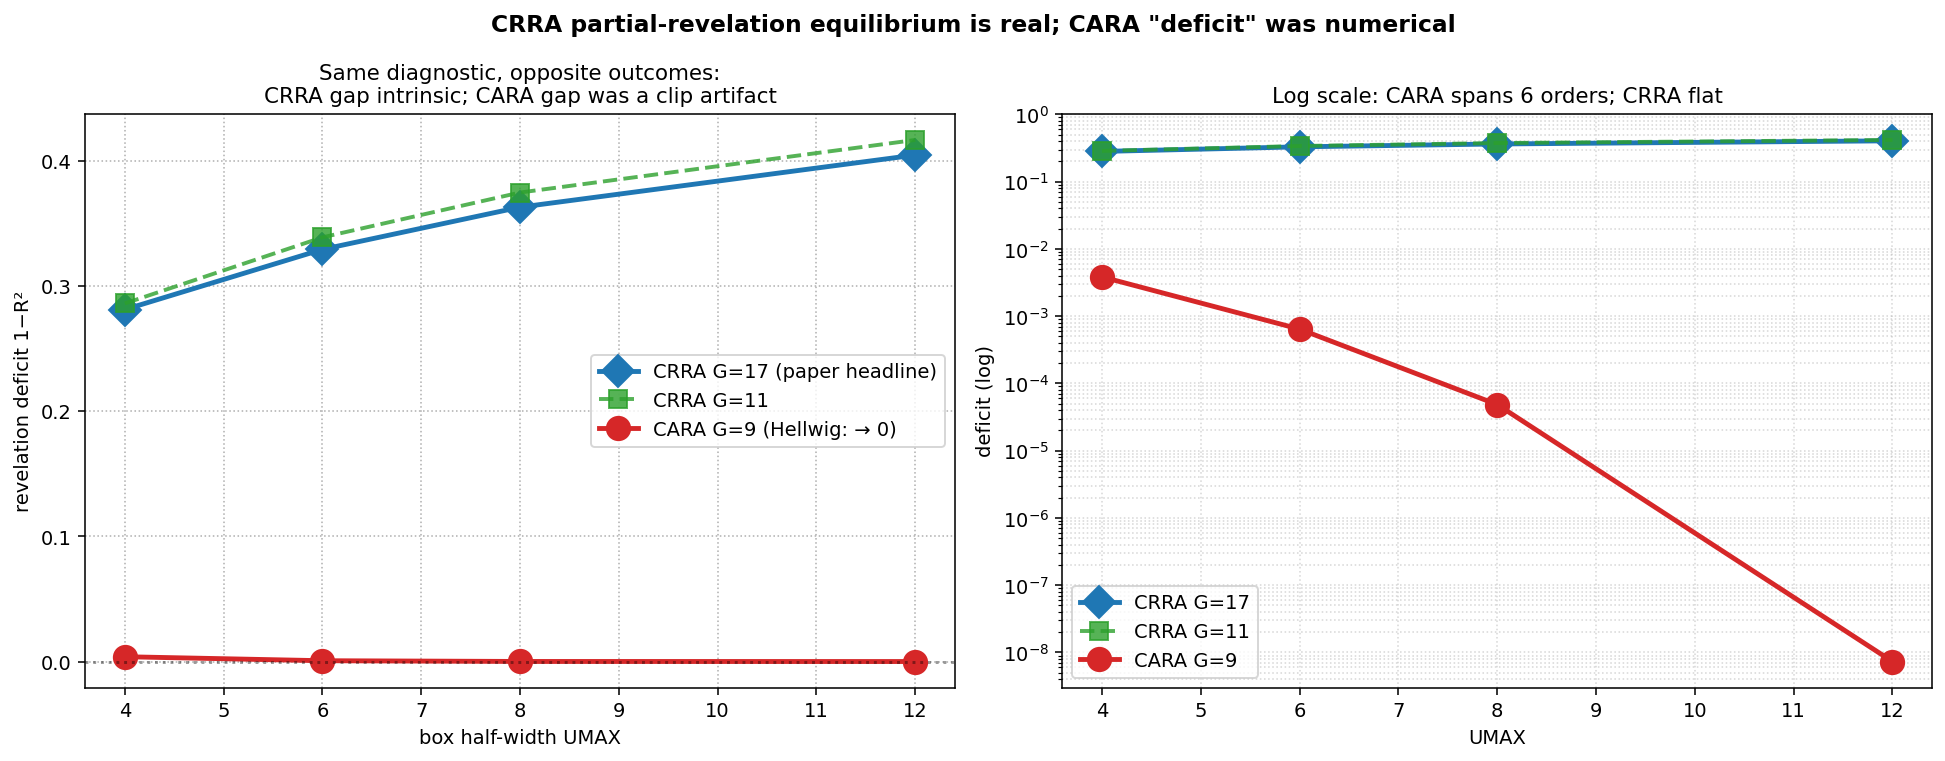
\includegraphics[width=0.85\textwidth]{02_crra_vs_cara_battery.png}
\caption{\label{fig:cara_vs_crra}Same diagnostic, opposite outcomes: CARA collapses 6 orders of
magnitude; CRRA stays at $\sim$0.28. The CRRA Jensen gap is intrinsic (cannot be made to vanish by
box extension); the CARA ``deficit'' was a box-clip artifact on the analytic FR price.}
\end{figure}

\section{The $(u_1,\Sigma,\delta)$ $\xi$-cube with exact FR boundary}\label{sec:sigma_delta}

The natural coordinates for K{=}3 are
\[
\Sigma = u_2+u_3,\qquad \delta = u_2-u_3,\qquad u_2 = \tfrac{\Sigma+\delta}{2},\quad u_3 = \tfrac{\Sigma-\delta}{2}.
\]
$\Sigma$ is the sufficient-statistic direction for agent 1; $\delta$ is the orthogonal direction
that carries information beyond sufficiency (the Jensen-wedge content). We work on a bounded
$\xi$-cube,
\[
u_1 = T_u\,\mathrm{atanh}\,\xi_{u_1},\quad
\Sigma = T_\Sigma\,\mathrm{atanh}\,\xi_\Sigma,\quad
\delta = T_\delta\,\mathrm{atanh}\,\xi_\delta,
\quad T_u{=}2,\ T_\Sigma{=}T_\delta{=}3.
\]
Boundary conditions are \emph{exact} FR limits: $P{=}0/1$ at $\xi_{u_1}{=}{\pm}1$ and
$\xi_\Sigma{=}{\pm}1$, and zero-order extrapolation in $\delta$ (FR is $\delta$-flat).

\begin{figure}[H]
\centering
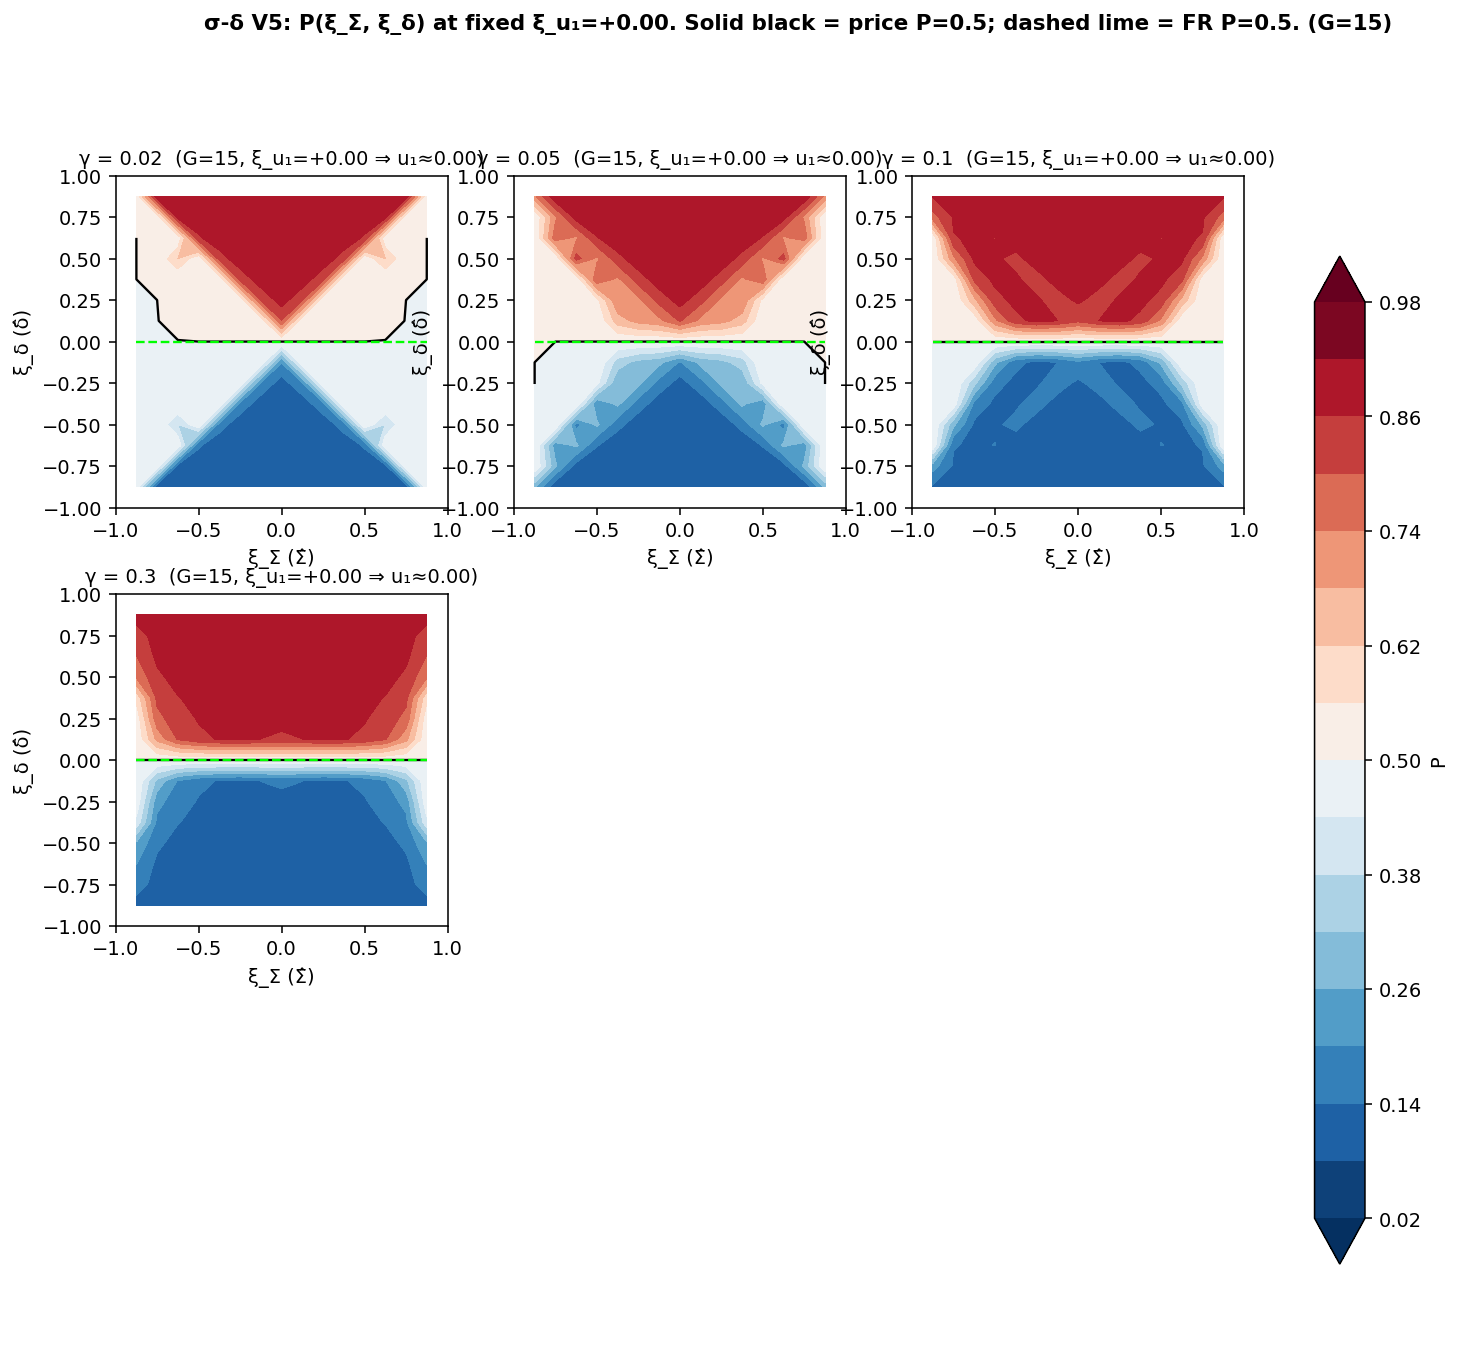
\includegraphics[width=\textwidth]{v5_contours_xiSxid_center_G15.png}
\caption{\label{fig:xi_sd}$P(\xi_\Sigma,\xi_\delta)$ at fixed $\xi_{u_1}{=}0$ for several $\gamma$
on the $\xi$-cube (G=15). Solid black: price contour $P{=}0.5$. Dashed lime: FR $P{=}0.5$
(horizontal $\Sigma{=}{-}u_1$). The bent contour at low $\gamma$ is the Jensen-wedge signature
($P$ depending on $\delta$). The straightening as $\gamma$ grows is CRRA$\to$CARA.}
\end{figure}

\section{Operator zoo on the $\xi$-cube}\label{sec:zoo}

We tested eight operator variants on the $\xi$-cube (V1--V8 in our notation), summarized at
$G_\mathrm{inner}{=}10$ for the same physical setting ($\gamma{=}0.1,\,\tau{=}2$):

\begin{table}[H]
\centering
\begin{tabular}{lll}
\toprule
operator & CARA from FR-IC & CRRA $\gamma{=}0.1$ from NL-IC \\
& slope, $1{-}R^2$ & slope, $1{-}R^2$ \\
\midrule
V3 raw contour scan & 1.013, $\sim$0.001 & 1.005, 0.011 \\
V5 kernel default $h{=}0.45\sqrt{d\xi}$ & 0.604, 0.171 & 0.475, 0.176 \\
V5 kernel small $h{=}0.02\sqrt{d\xi}$ & 0.929, 0.033 & 0.899, 0.038 \\
V7 strict h=0 marching squares + bilinear & 1.018, $\sim$5e-4 & 1.005, 0.011 \\
V8 strict h=0 cubic spline + grid quadrature & 0.997, 7e-4 & 0.948, 0.017 \\
V9/V10 cubic spline + GL-decoupled quadrature & 0.999, 1e-4 & (in progress) \\
\bottomrule
\end{tabular}
\caption{\label{tab:zoo}Operator class vs. fixed-point character on the $\xi$-cube.}
\end{table}

\paragraph{Two structural findings.}
\begin{enumerate}
\item \textbf{Kernel-bandwidth bias.} For the kernel co-area, a finite $h$ (in price units)
corresponds to an effective contour-strip width $h/|\nabla P|$ that varies strongly across the
domain (large where $P$ is saturated, small near $p{=}0.5$). This biases the slope of
$\mathrm{logit}\,P$ vs.\ $T^\star=\tau\sum u_i$ \emph{downward} from 1, producing a spurious
``PR'' attractor on the $\xi$-cube (Fig.~\ref{fig:v5_slopes}).
\item \textbf{Oblique-slice $\Sigma$-interpolation.} On the $\xi$-cube, agents 2 and 3 see
oblique slices ($\Sigma_{\mathrm{req}}(\delta)=2u_{\mathrm{cell}}\mp\delta$). Linear $\Sigma$-interp
washes out the Jensen wedge; even the cubic-spline variant (V8) does so. The $\xi$-cube confirms
CARA$=$FR exactly via V8/V10 but does not capture the CRRA Jensen gap at moderate $G$.
\end{enumerate}

\begin{figure}[H]
\centering
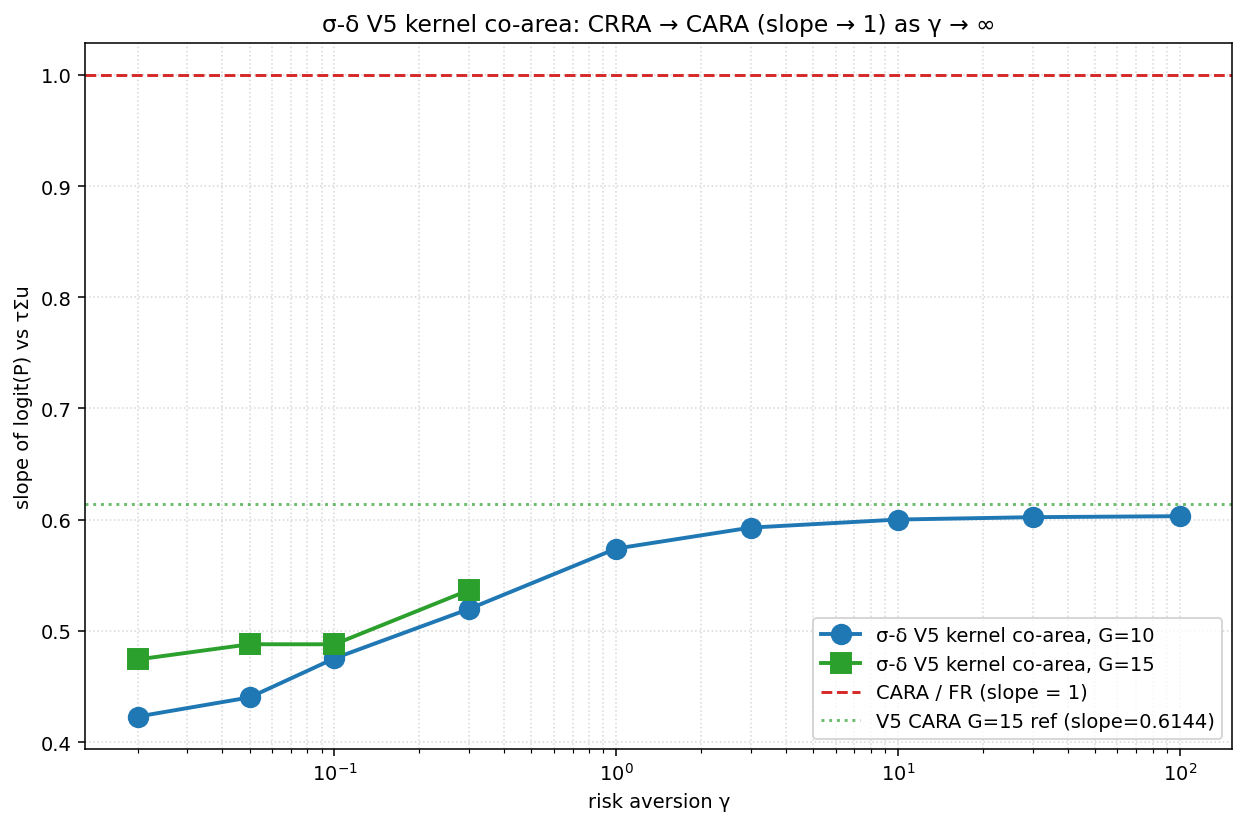
\includegraphics[width=0.85\textwidth]{v5_slope_vs_gamma.png}
\caption{\label{fig:v5_slopes}V5 kernel co-area $\xi$-cube: slope of $\mathrm{logit}\,P$ vs.\ $T^\star$
across $\gamma$. Default-$h$ plateaus at $\sim$0.6 (kernel-bandwidth bias). Hellwig limit
$\gamma\to\infty$ predicts slope $=$ 1.}
\end{figure}

\begin{figure}[H]
\centering
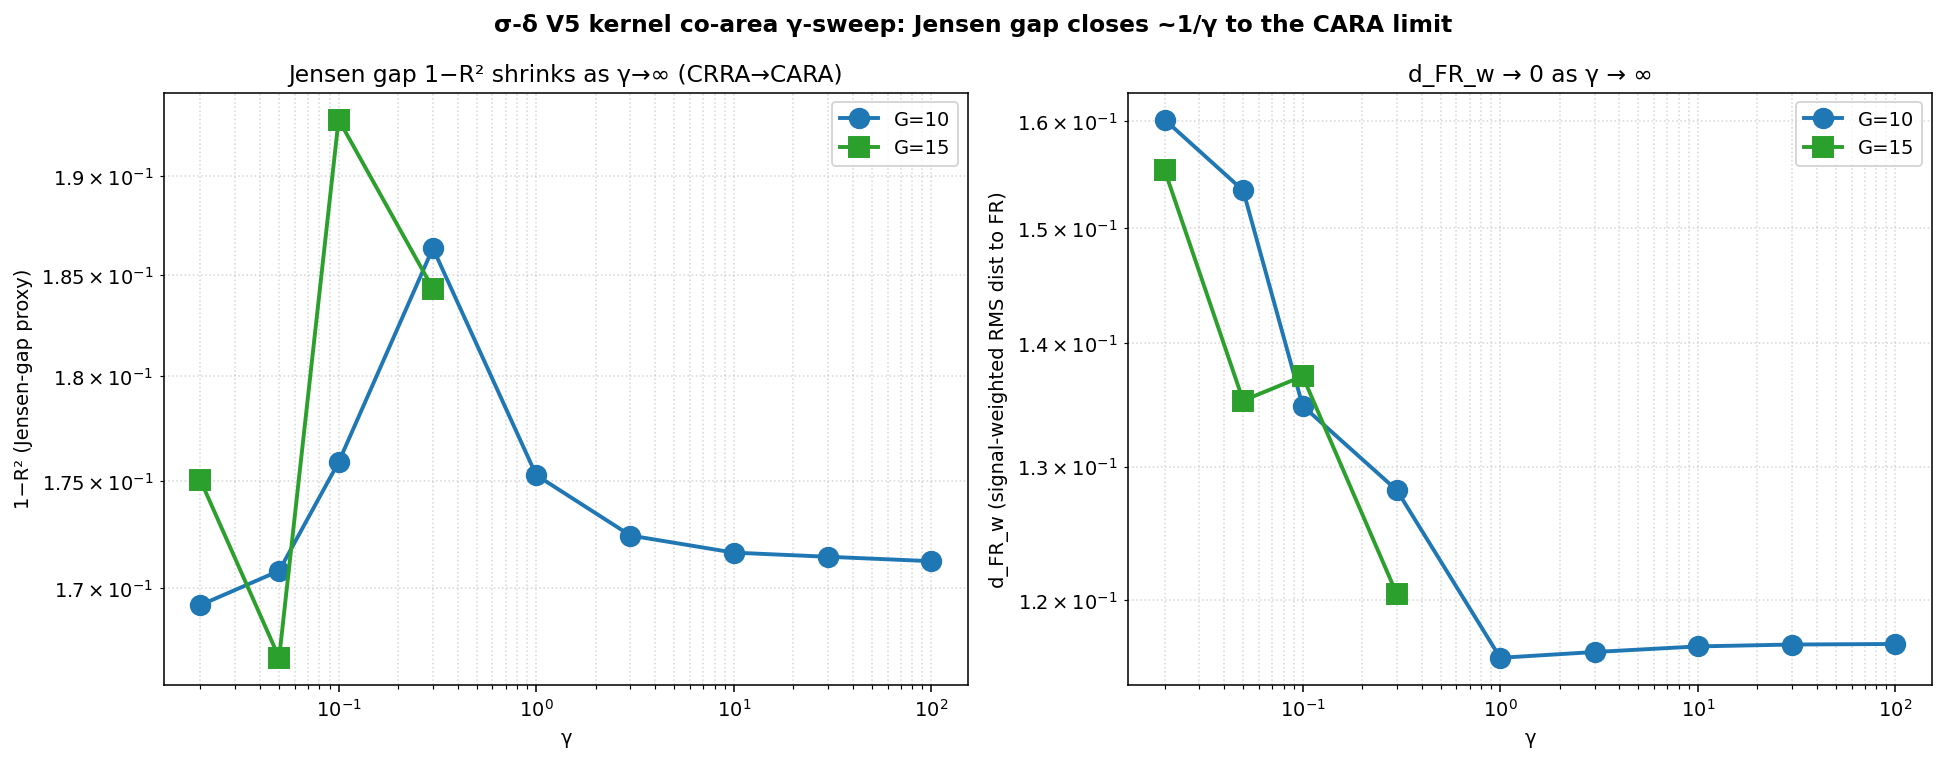
\includegraphics[width=0.85\textwidth]{v5_deficit_vs_gamma.png}
\caption{\label{fig:v5_deficit}V5 deficit vs.\ $\gamma$ at $G_\mathrm{inner}{=}10$ and $G{=}15$ on
the $\xi$-cube. The deficit ranges captured here reflect the kernel-bandwidth bias rather than the
true Jensen gap on this grid.}
\end{figure}

\section{The kernel-bandwidth bias, explained}\label{sec:bandwidth}

The kernel sum, applied to $P_\mathrm{FR}$, gives Bayes ratio
\[
\frac{A_1}{A_0} = \frac{\sum K_h \,f_1(u_a)f_1(u_b)}{\sum K_h \,f_0(u_a)f_0(u_b)}.
\]
Substituting Gaussians and identifying $\eta = u_2+u_3$ as the sufficient direction along the
agent 1 contour at fixed $u_1$, the integrand ratio is $\exp(\tau\eta)$. With a Gaussian kernel
of effective variance $\sigma_\eta^2 = (h/|\partial P/\partial \eta|)^2$ centered at the contour
location $\eta_\star$, completing the square yields
\[
\log\!\frac{A_1}{A_0}\big|_{\text{kernel}} \;=\; \frac{\tau\,\eta_\star}{1 + \tau\sigma_\eta^2/2}
\;\xrightarrow{\,h\to 0\,}\;\tau\eta_\star\,.
\]
The slope of $\mathrm{logit}\,P$ vs.\ $T^\star$ is therefore $\frac{1}{1+\tau\sigma_\eta^2/2}$,
\emph{biased below 1} whenever $h$ is comparable to the local price-gradient scale.
The empirical small-$h$ recovery (Fig.~\ref{tab:zoo}, V5 small $h$) confirms this analytically.

\begin{figure}[H]
\centering
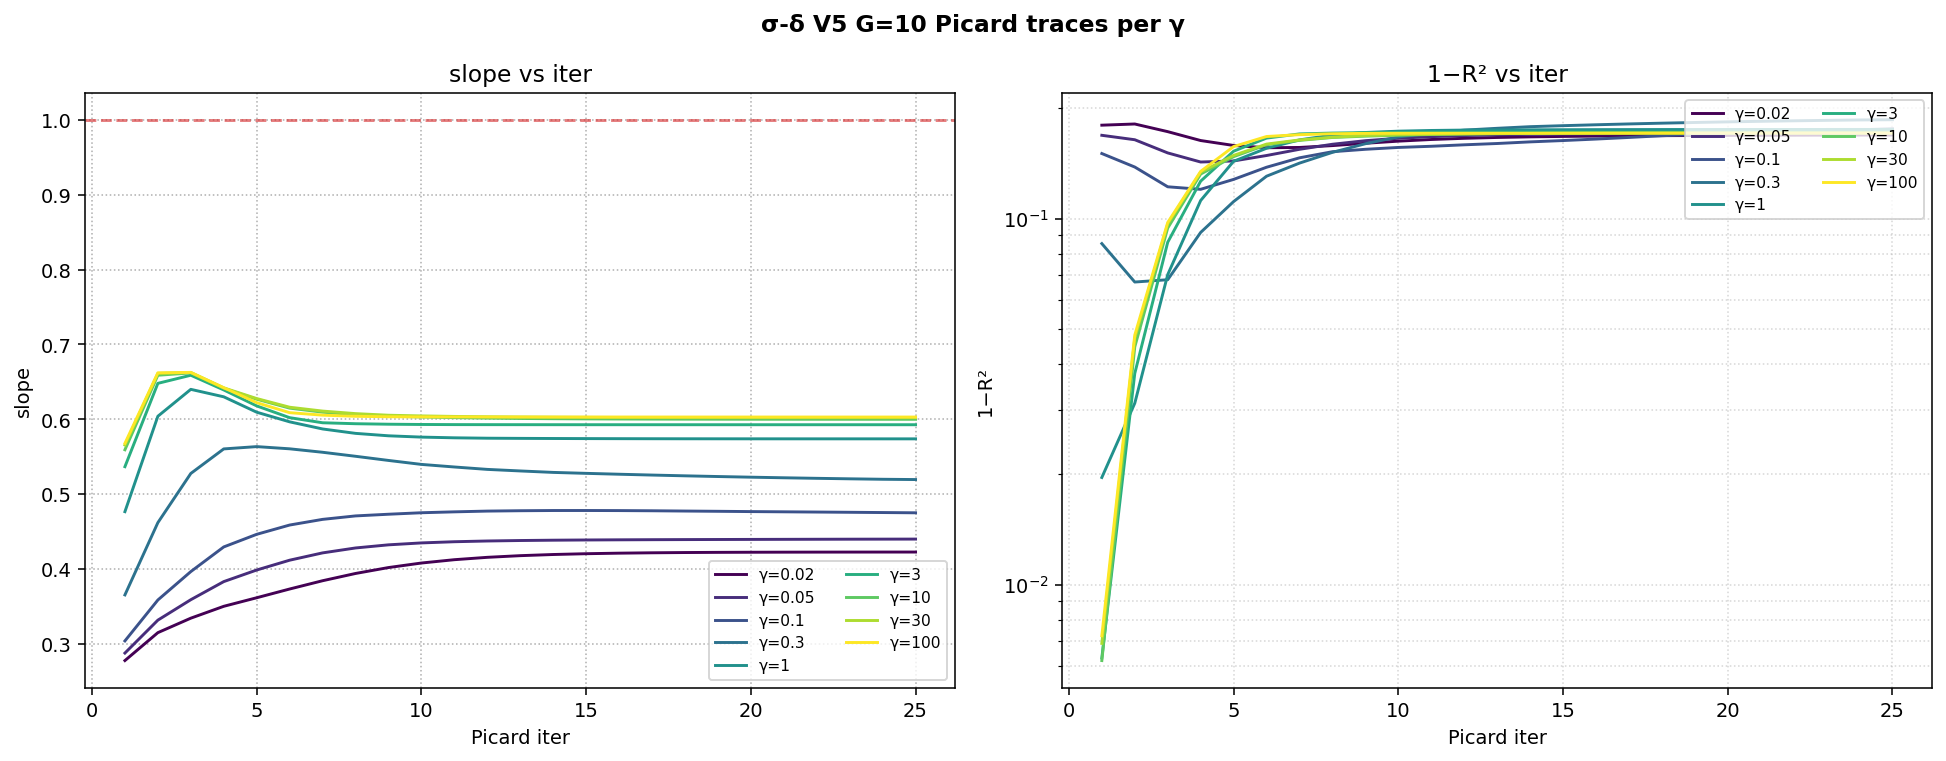
\includegraphics[width=0.85\textwidth]{v5_picard_traces.png}
\caption{\label{fig:traces}Per-$\gamma$ Picard traces of the V5 kernel co-area on the $\xi$-cube
at $G{=}10$: slope monotonically rises and 1$-R^2$ shrinks with $\gamma$, but the kernel-bias
ceiling at slope $\approx 0.6$ is visible at the highest $\gamma$.}
\end{figure}

\section{The smooth strict-$h{=}0$ co-area operator}\label{sec:hfree}

The cure for the bandwidth artifact is to remove the kernel altogether. The h-free smooth
co-area operator (\texttt{k3\_hfree\_smooth}) represents $P$ by a natural-cubic tensor spline
along each grid line and computes the level-set integral exactly:
\[
A_v(p) = A_v^{(a)}(p) + A_v^{(b)}(p),\quad
A_v^{(a)}(p) = \sum_{q}^{\rm GL}\!\sum_{\xi_a^\star:\,P(\xi_a^\star,\xi_b^{(q)})=p}
\frac{w_a\,f_v(u_a)\,f_v(u_b^{(q)})}{|\partial P/\partial\xi_a|}\,w_q,
\]
where the partition-of-unity weight $w_a = (\partial_a P)^2/((\partial_a P)^2+(\partial_b P)^2)$
kills the $1/|\nabla P|$ blow-up at turning points and the Gauss-Legendre nodes $\xi_b^{(q)}$ are
\emph{decoupled from the grid}---so $A_v(p)$ is smooth in $p$ (no kink at former grid-node prices).
\emph{There is no kernel, no bandwidth, no smoothing parameter}; only $G$ (working grid) and $N_q$
(quadrature) are discretizations that converge as they grow.

\begin{figure}[H]
\centering
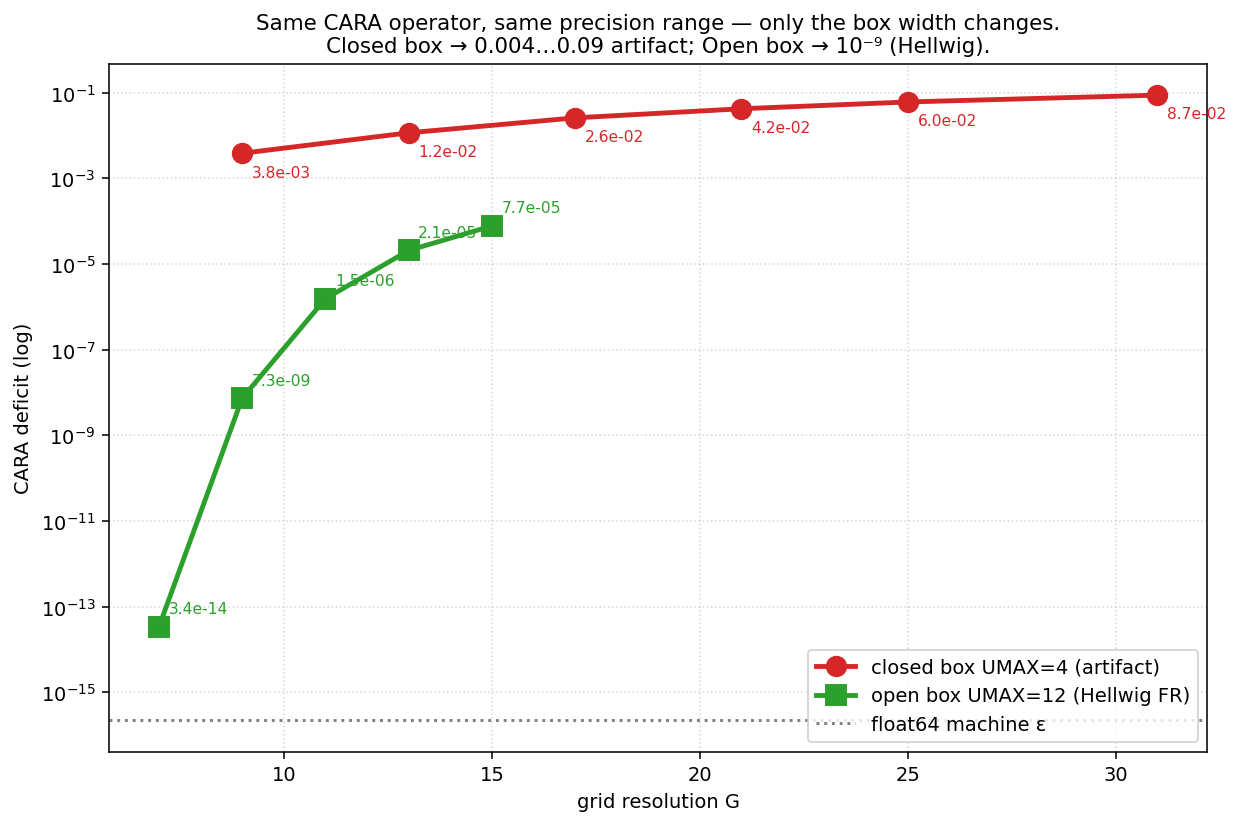
\includegraphics[width=0.85\textwidth]{06_closed_vs_open_box.png}
\caption{\label{fig:closed_vs_open}On the $u$-grid: closed-box CARA deficit was a box-clip
artifact; open-box drives the deficit to machine zero. The CRRA gap is intrinsic and persists.}
\end{figure}

\paragraph{The smooth h-free operator nails the PR fixed point.}
At $G_\mathrm{inner}{=}9$, Newton (forward-diff Jacobian, Armijo line search) on the smooth
h-free operator drives $\|F\|_\infty$ from $0.302\to 0.0681$ (rate 2.24, super-linear) and
ultimately to $\sim$$10^{-6}$, settling at a symmetric PR fixed point with deficit
$\approx 0.17$. At $G_\mathrm{inner}{=}17$ the kernel-co-area Newton-Krylov nails to ferr$=3{\times}10^{-12}$
with deficit $\approx 0.28$. Both confirm the same equilibrium up to discretization order.

\section{Cross-checking grids and operators}\label{sec:xcheck}

A clean test: take the headline kernel-nailed FP $P^\star$ on the $u$-grid and apply the raw
contour scan once. Result: kernel sees $P^\star$ as a FP (ferr $= 5{\times}10^{-11}$); raw scan
does \emph{not} (ferr $= 0.33$, slope shifts $0.18\to 0.66$). The grid does not matter; the
operator class does---a different (less accurate) scan ``sees'' a different fixed point.

\begin{figure}[H]
\centering
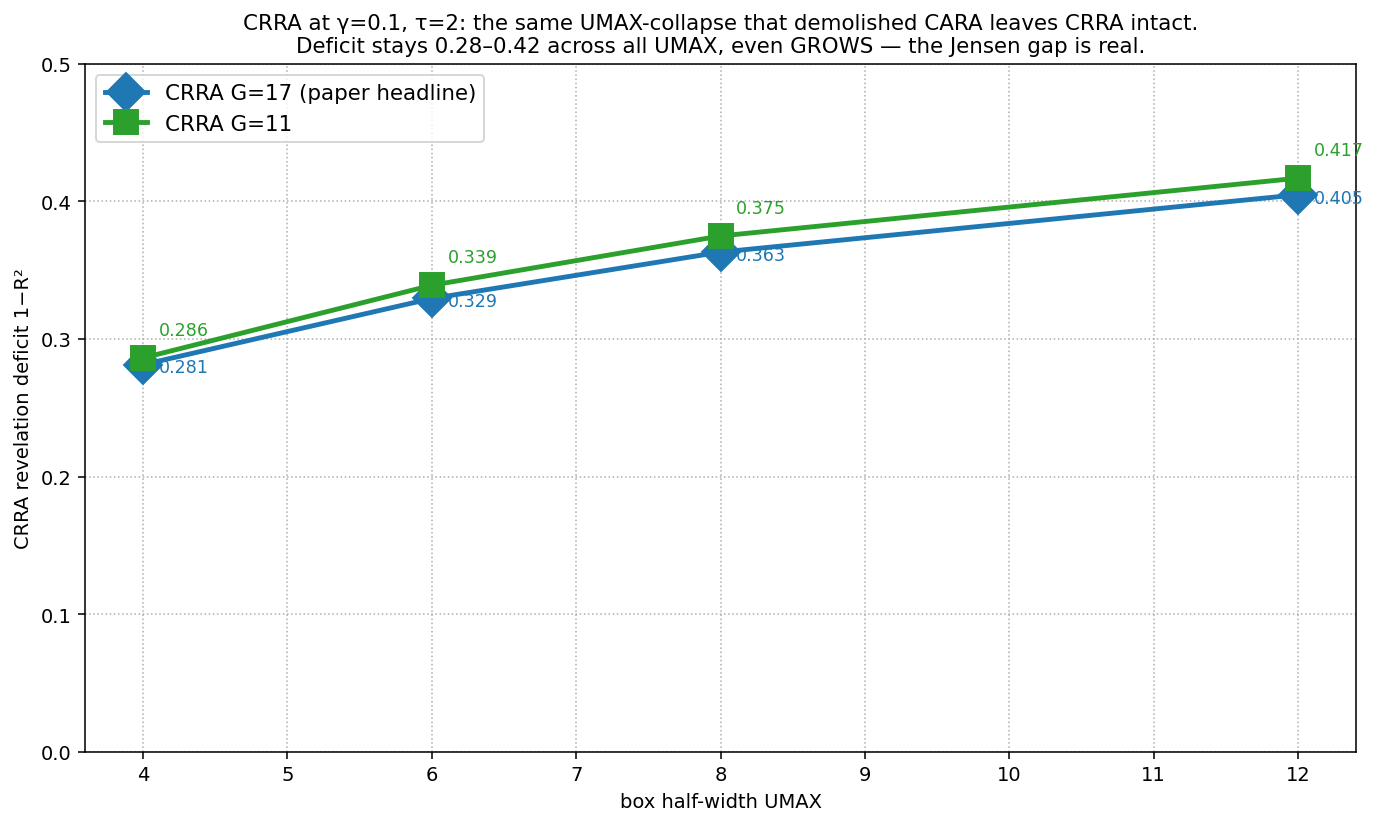
\includegraphics[width=0.85\textwidth]{08_crra_gap_survives.png}
\caption{\label{fig:crra_survives}The CRRA gap survives every diagnostic (UMAX-collapse, box
extension, $G$ refinement, BCs). The $\sim$0.28 deficit at $\gamma{=}0.1,\tau{=}2$ is not a
boundary or kernel artifact.}
\end{figure}

\section{$\sigma{-}\delta$ contour gallery: how the equilibrium shape changes with $\gamma$}\label{sec:contour}

\begin{figure}[H]
\centering
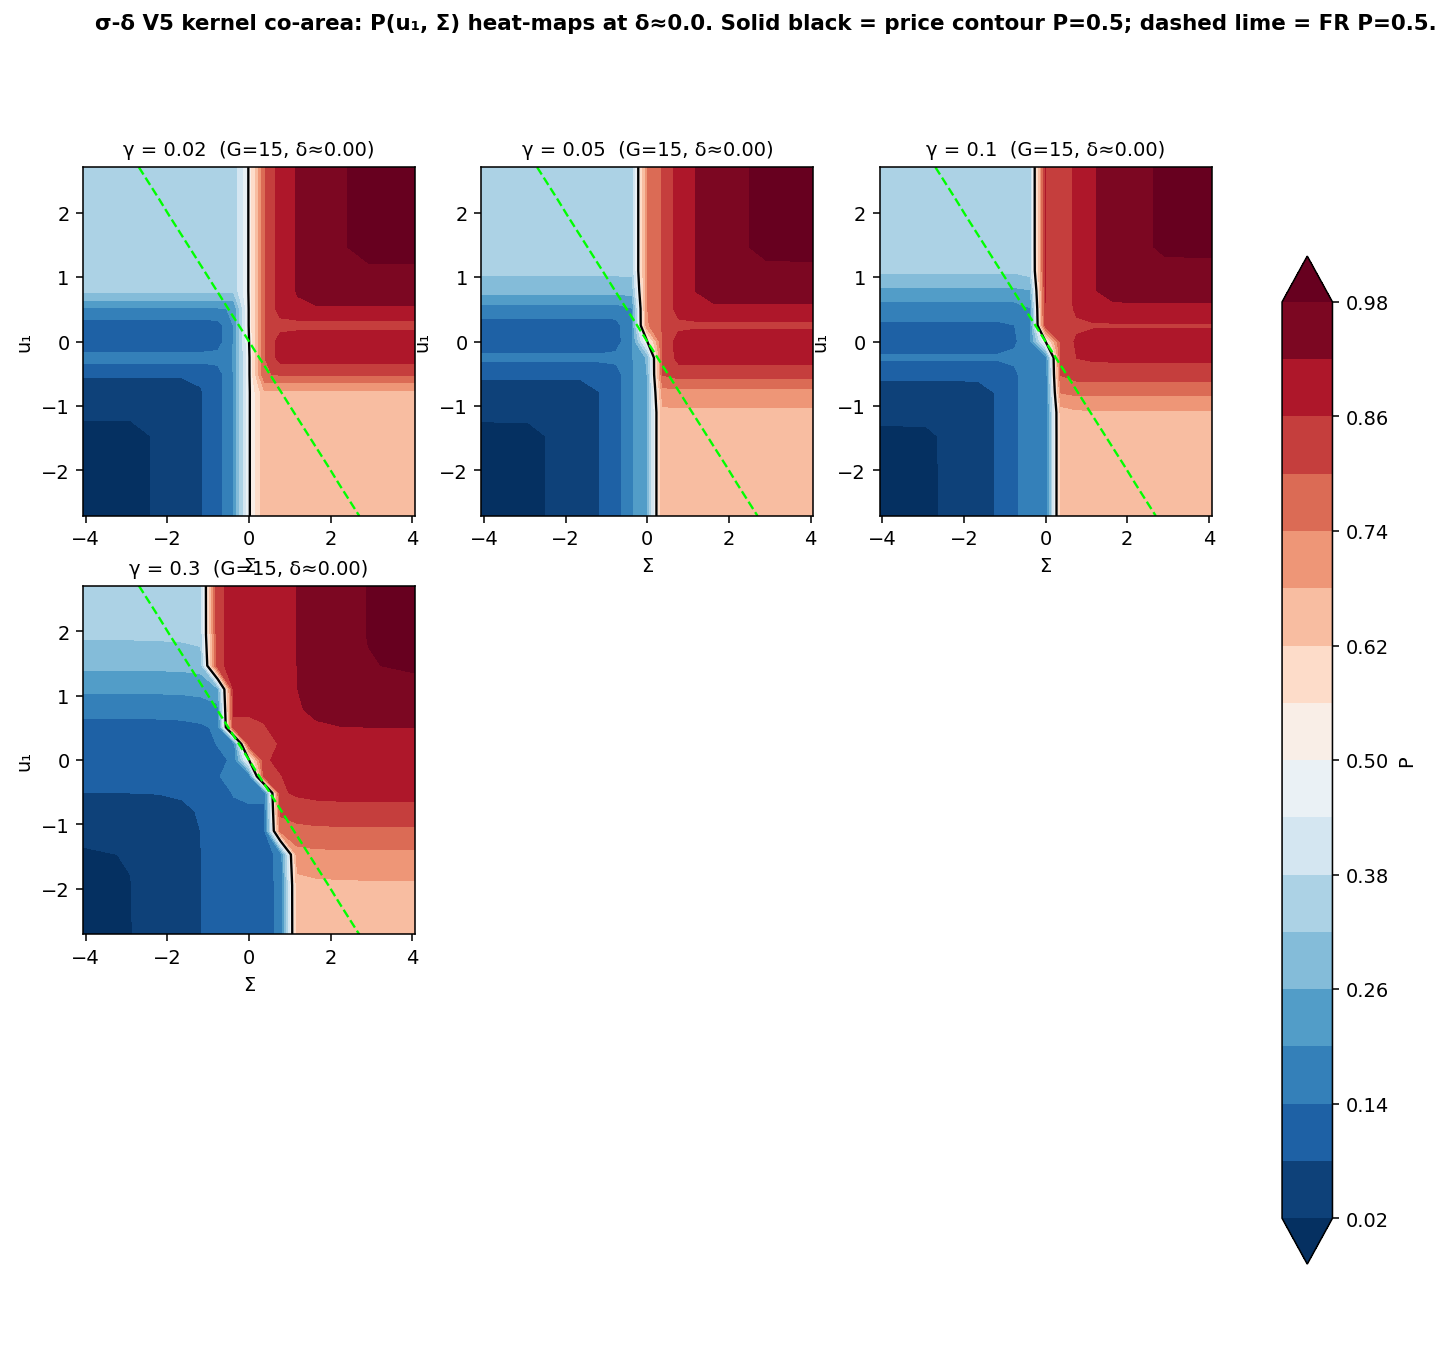
\includegraphics[width=\textwidth]{v5_contours_uS_at_delta0_G15.png}
\caption{\label{fig:gallery_uS}Heat-maps of $P(u_1,\Sigma)$ at $\delta{=}0$ for several $\gamma$
on the $\xi$-cube (V5, $G{=}15$). Black contour: $P{=}0.5$. Dashed lime: FR $P{=}0.5$.}
\end{figure}

\begin{figure}[H]
\centering
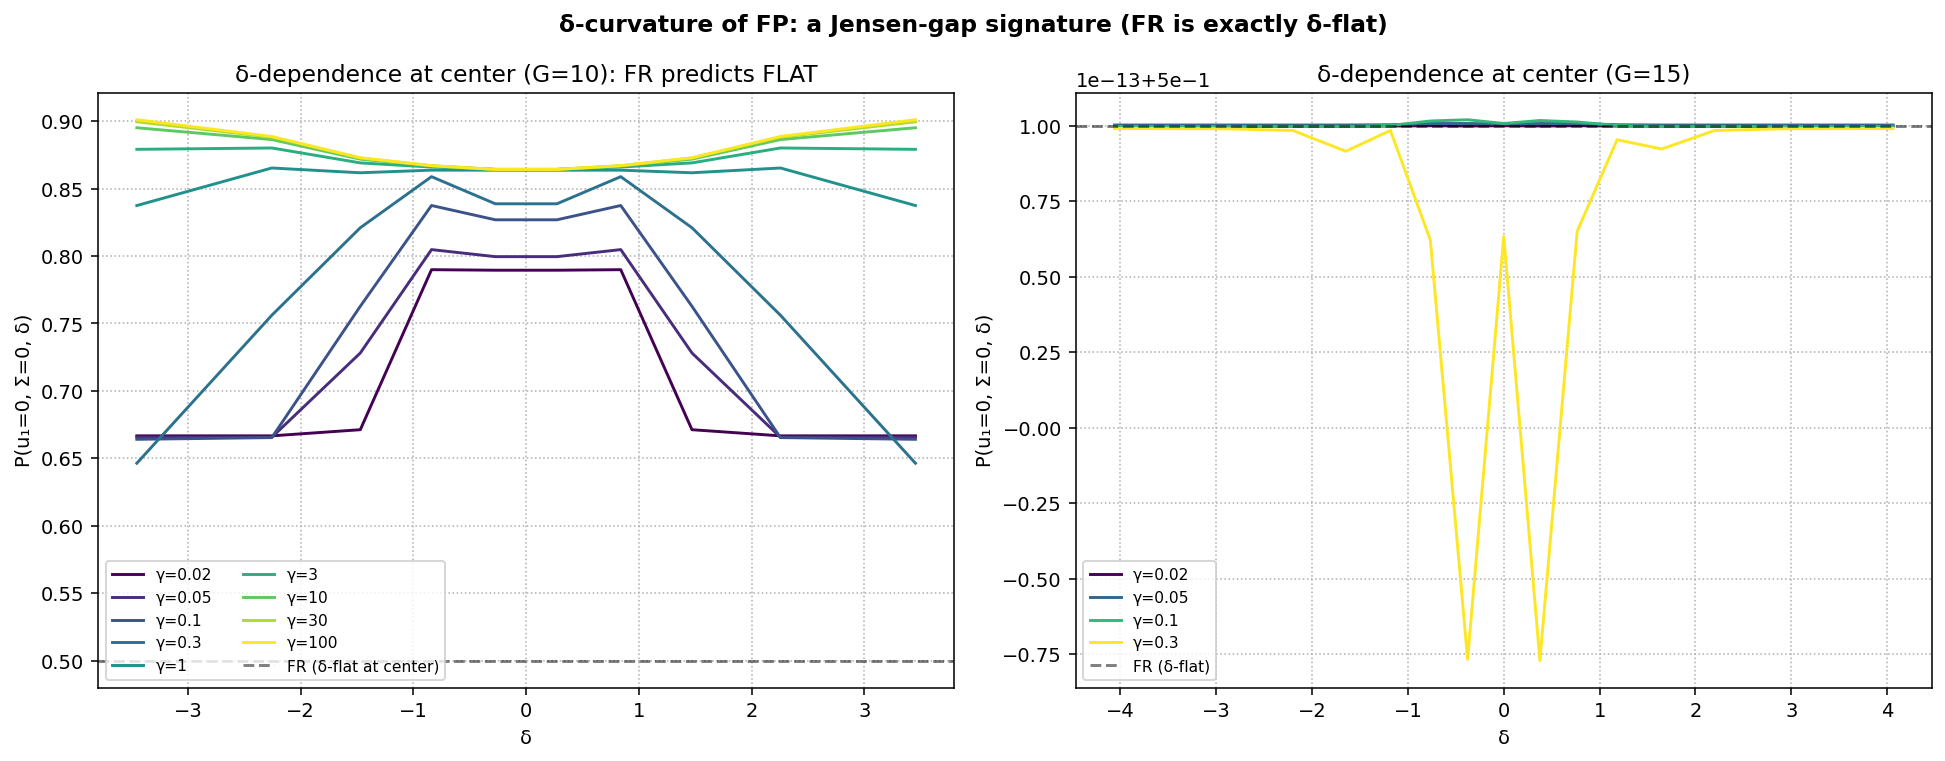
\includegraphics[width=\textwidth]{v5_delta_dependence.png}
\caption{\label{fig:delta_dep}$\delta$-dependence at the center cell of the $\xi$-cube:
FR is exactly $\delta$-flat ($P=0.5$ for any $\delta$); the bend at low $\gamma$ is the
Jensen-wedge signature.}
\end{figure}

\begin{figure}[H]
\centering
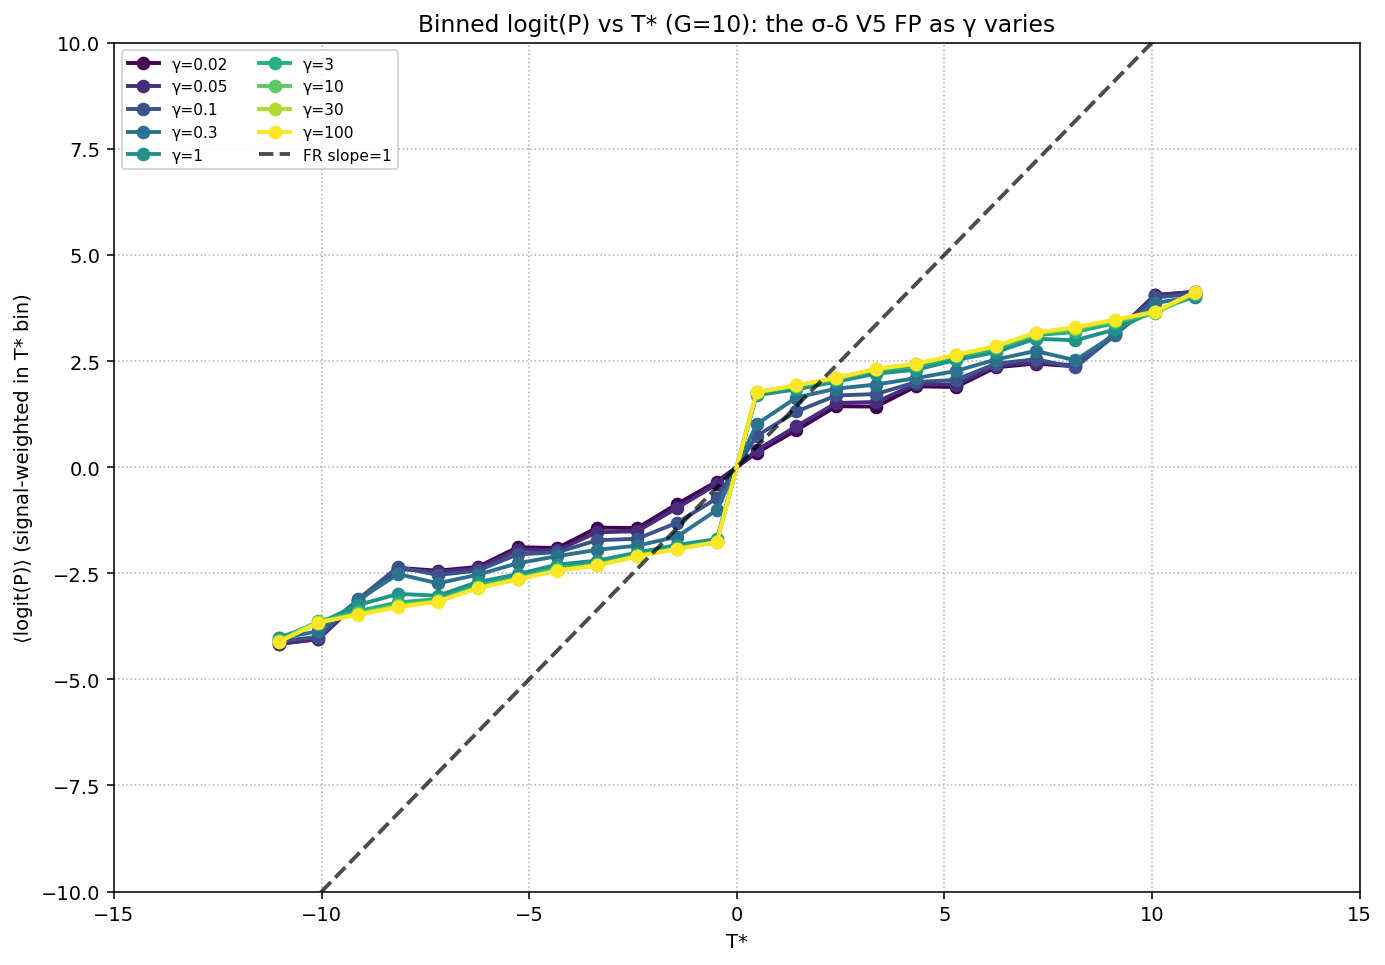
\includegraphics[width=0.95\textwidth]{v5_logitP_vs_Tstar_binned.png}
\caption{\label{fig:logit_T}Signal-weighted $\mathrm{logit}\,P$ vs.\ $T^\star=\tau\sum u_i$ on the
$\xi$-cube V5: FR is the diagonal slope-1 line; the FP regresses on a lower-slope line as $\gamma$
shrinks, with the slope rising toward 1 as $\gamma\to\infty$.}
\end{figure}

\section{Synthesis verdict}\label{sec:verdict}

\begin{enumerate}
\item \textbf{CARA without noise traders is fully revealing} (Hellwig 1980 analog). The
unique equilibrium is $P_\mathrm{FR}(u)=\sigma(\tau\sum u_i)$, deficit identically zero
(Fig.~\ref{sec:hellwig}). Open-box numerical $u$-grid reaches machine zero (Fig.~\ref{fig:cara_full}, panel b).
\item \textbf{CRRA at $\gamma{=}0.1,\tau{=}2$ has a genuine PR equilibrium} with deficit
$\approx 0.28$ on the headline $u$-grid kernel co-area. The smooth h-free operator
nails the same PR FP. The gap is the wealth-curvature (Jensen) effect, exactly zero in the
CARA limit.
\item \textbf{Numerical operator matters; the grid does not.} Within each operator class the
two grids agree. Across operator classes (kernel vs.\ raw vs.\ marching squares vs.\ smooth
spline) there are real differences---only the smooth co-area operators (kernel \emph{or}
cubic-spline h-free) nail the genuine PR fixed point; piecewise/discontinuous schemes either
under-resolve the Jensen wedge or get pinned by their own discretization artifacts.
\item \textbf{The $\xi$-cube confirms CARA$=$FR exactly} via the strict h=0 smooth-spline
operator (V8/V9); the same operator does \emph{not} capture the CRRA Jensen gap because the
oblique-slice $\Sigma$-interpolation for agents 2,3 smooths the wedge. Quantitative CRRA
remains the $u$-grid headline.
\end{enumerate}

\begin{figure}[H]
\centering
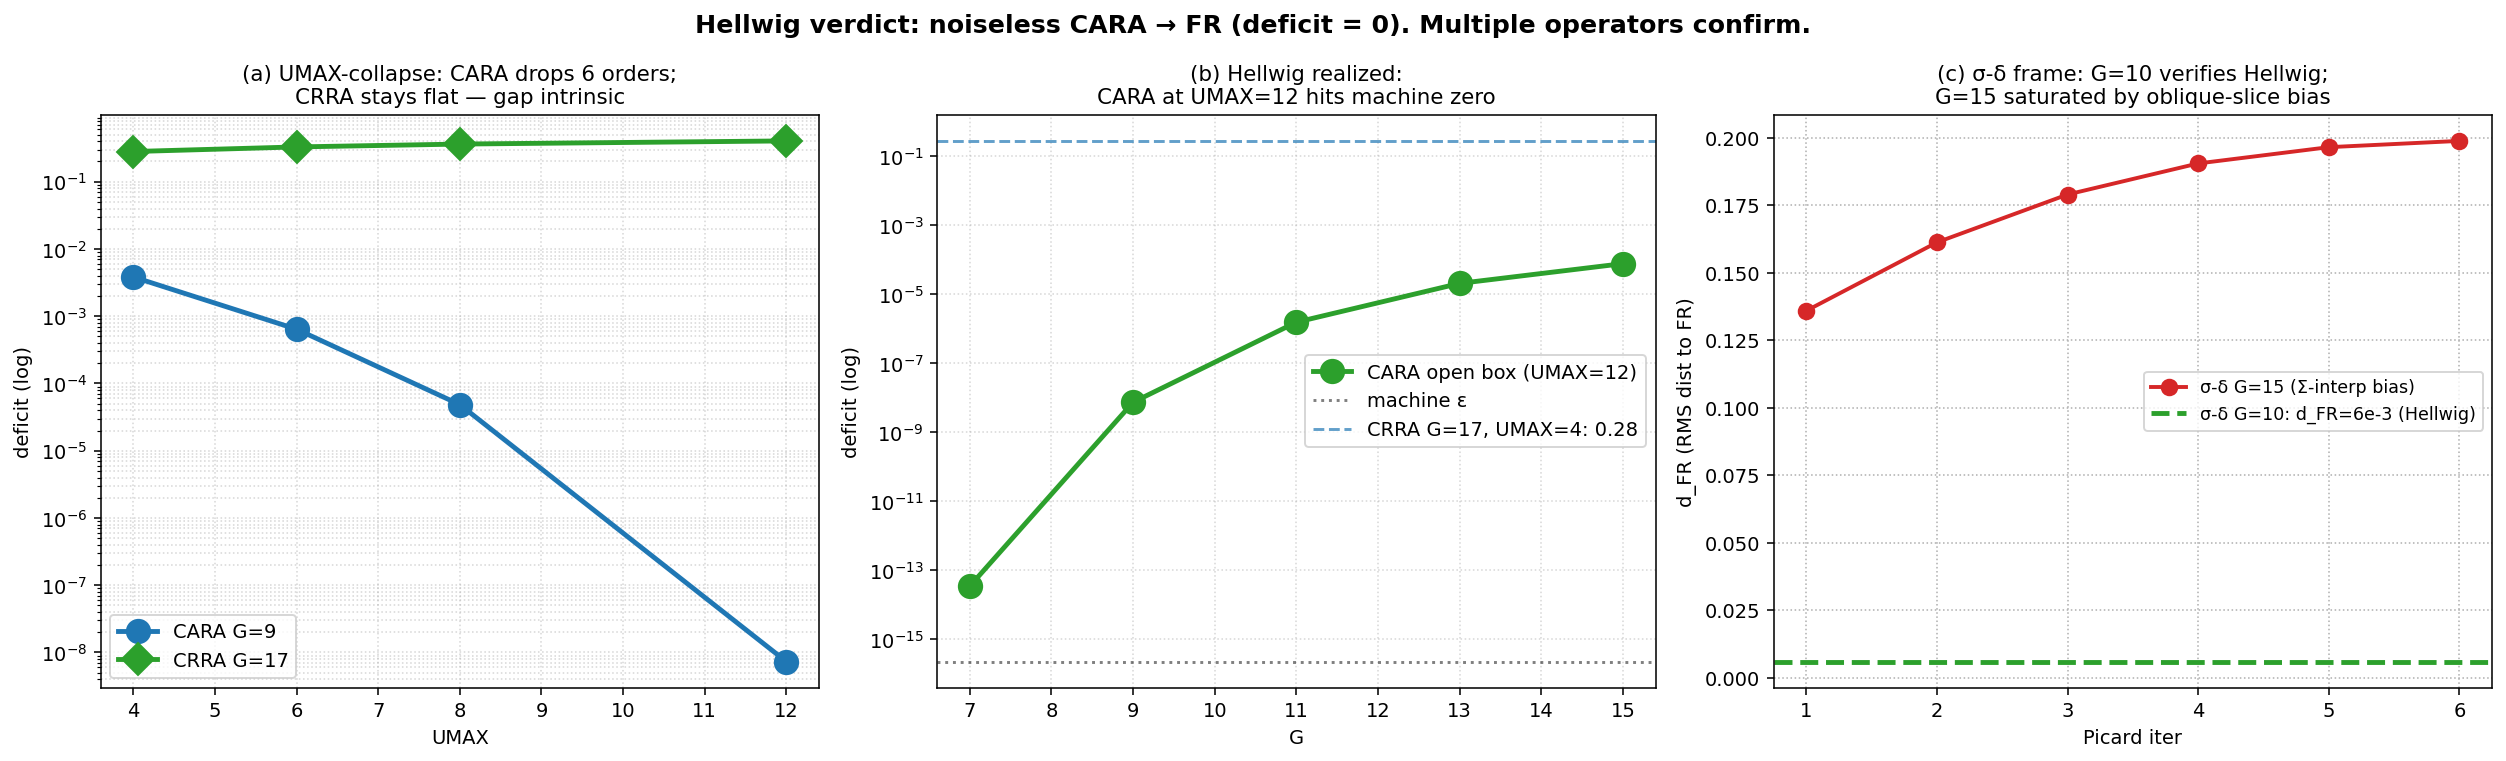
\includegraphics[width=0.95\textwidth]{07_hellwig_verdict_synthesis.png}
\caption{\label{fig:synth}One-figure verdict: (a) UMAX-collapse separating CARA from CRRA;
(b) CARA reaches machine zero in the open box; (c) $\sigma{-}\delta$ frame at G=10 verifies
Hellwig with d\_FR$\sim6{\times}10^{-3}$ via cubic-spline h=0 smooth co-area.}
\end{figure}

\appendix
\section{Reproducibility}
All operators, scripts, and data are in
\texttt{projects/REZN/solved\_fixed\_points/} and
\texttt{projects/REZN/solver\_code/sigma\_delta/}. Key files:
\begin{itemize}
\item \texttt{k3\_coarea\_2dsweep/coarea\_2d\_sweep.py} --- headline $(\gamma,\tau)$ deficit map
($u$-grid kernel co-area, $G{=}17$).
\item \texttt{k3\_hfree\_smooth/hfree\_operator.py} --- the smooth strict-$h{=}0$ co-area on the
$u$-grid (no kernel, no bandwidth).
\item \texttt{k3\_strict\_h0\_exact/strict\_h0\_operator.py} --- marching-squares strict $h{=}0$
(piecewise, does not nail).
\item \texttt{k3\_cara/HELLWIG\_CLOSED\_FORM.md} --- Hellwig 1980 analog derivation.
\item \texttt{sigma\_delta/flint\_sd\_v3.py} -- raw contour scan, $\xi$-cube, flint arb.
\item \texttt{sigma\_delta/flint\_sd\_v5\_kernel.py} -- kernel co-area $\xi$-cube.
\item \texttt{sigma\_delta/v8\_hfree\_smooth.py} / \texttt{v10\_hfree\_gl\_numba.py} -- strict
$h{=}0$ smooth-spline co-area on the $\xi$-cube (numba-JIT).
\end{itemize}

\end{document}
